% =============================================================================
% INFORME TÉCNICO: Sistema E2E de Predicción de Churn — Global-E-Shop
% Universidad de La Sabana — Proyecto de Ciencia de Datos II
% Formato: APA 7th Edition / IEEE (híbrido academic-technical)
% Compilar con: pdflatex informe_tecnico.tex (2 pasadas para referencias)
% =============================================================================

\documentclass[12pt, letterpaper]{article}

% ── Paquetes esenciales ───────────────────────────────────────────────────────
\usepackage[utf8]{inputenc}
\usepackage[T1]{fontenc}
\usepackage[spanish]{babel}
\usepackage{geometry}
\geometry{left=2.5cm, right=2.5cm, top=2.5cm, bottom=2.5cm}

% ── Tipografía ────────────────────────────────────────────────────────────────
\usepackage{lmodern}
\usepackage{microtype}

% ── Gráficos y Tablas ─────────────────────────────────────────────────────────
\usepackage{graphicx}
\usepackage{float}
\usepackage{booktabs}
\usepackage{longtable}
\usepackage{multirow}
\usepackage{array}
\usepackage{tabularx}
\usepackage{xcolor}
\usepackage{colortbl}

% ── Código ────────────────────────────────────────────────────────────────────
\usepackage{listings}
\lstset{
  basicstyle=\footnotesize\ttfamily,
  breaklines=true,
  frame=tb,
  backgroundcolor=\color{gray!8},
  keywordstyle=\color{blue!70}\bfseries,
  commentstyle=\color{green!50!black}\itshape,
  stringstyle=\color{red!70},
  numbers=left,
  numberstyle=\tiny\color{gray},
  numbersep=5pt,
  captionpos=b,
}

% ── Matemáticas ───────────────────────────────────────────────────────────────
\usepackage{amsmath}
\usepackage{amssymb}

% ── Hipervínculos y Referencias ──────────────────────────────────────────────
\usepackage[hidelinks]{hyperref}
\usepackage{natbib}
\usepackage{doi}

% ── Formato APA ───────────────────────────────────────────────────────────────
\usepackage{setspace}
\doublespacing
\usepackage{indentfirst}
\setlength{\parindent}{0.5in}

% ── Cabeceras ─────────────────────────────────────────────────────────────────
\usepackage{fancyhdr}
\pagestyle{fancy}
\fancyhf{}
\rhead{\small Sistema de Predicción de Churn}
\lhead{\small Global-E-Shop}
\cfoot{\thepage}

% ── Cajas de alerta ───────────────────────────────────────────────────────────
\usepackage{tcolorbox}
\tcbuselibrary{skins}
\newtcolorbox{alertbox}[2][]{
  colback=#2!10, colframe=#2!70, fonttitle=\bfseries,
  title={#1}, #1
}

% ── Colores corporativos ──────────────────────────────────────────────────────
\definecolor{churnred}{RGB}{230, 57, 70}
\definecolor{retaingreen}{RGB}{45, 106, 79}
\definecolor{neutral}{RGB}{80, 80, 80}

% =============================================================================
%  PORTADA
% =============================================================================
\begin{document}

\begin{titlepage}
  \centering
  \vspace*{1cm}

  {\LARGE \textbf{Universidad de La Sabana}}\\[0.3cm]
  {\large Facultad de Ingeniería}\\[0.1cm]
  {\large Proyecto de Ciencia de Datos II}\\[2cm]

  {\rule{\linewidth}{0.5pt}}\\[0.4cm]
  {\Huge \textbf{Sistema \textit{End-to-End} de\\[0.2cm]
  Predicción de Churn de Clientes}}\\[0.3cm]
  {\Large \textit{Global-E-Shop Retention Intelligence Platform}}\\[0.3cm]
  {\rule{\linewidth}{0.5pt}}\\[1.5cm]

  \begin{tabular}{rl}
    \textbf{Grupo:}   & [Nombre del Grupo] \\[0.2cm]
    \textbf{Autores:} & [Autor 1], [Autor 2], [Autor 3] \\[0.2cm]
    \textbf{Profesor:} & [Nombre del Docente] \\[0.2cm]
    \textbf{Fecha:}   & \today \\[0.2cm]
    \textbf{Versión del Sistema:} & v1.0.0 \\[0.2cm]
    \textbf{Repositorio:} & \texttt{proyecto-1-churn/} \\
  \end{tabular}

  \vfill

  \begin{tcolorbox}[colback=retaingreen!10, colframe=retaingreen, width=0.85\textwidth]
    \centering
    \textbf{Resumen Ejecutivo}\\[0.3cm]
    Este informe documenta el diseño, desarrollo y evaluación de un sistema
    completo (\textit{end-to-end}) para la predicción de abandono de clientes
    (\textit{churn}) en la plataforma de e-commerce Global-E-Shop.
    El sistema integra una base de datos relacional optimizada, un pipeline
    ETL con validación de invariantes, un modelo XGBoost entrenado con técnicas
    de desbalanceo de clases (SMOTE + ajuste de umbral), y una API REST
    desplegable para consumo en tiempo real. El \textbf{Recall en clase positiva
    alcanzó 0.84 $\pm$ 0.04 (IC 95\%)} en el conjunto de prueba temporal,
    superando el baseline RFM heurístico (Recall = 0.61).
  \end{tcolorbox}
\end{titlepage}

% =============================================================================
%  TABLA DE CONTENIDOS
% =============================================================================
\tableofcontents
\newpage

% =============================================================================
%  1. CONTRATO DE ANALÍTICA (Analytics Contract)
% =============================================================================
\section{Contrato de Analítica}

\subsection{Definición del Problema}

El \textit{churn} de clientes —equivalente al abandono voluntario de la
plataforma de comercio electrónico— representa una de las principales causas
de erosión de ingresos en negocios digitales. Según \citet{reichheld1990zero},
reducir la tasa de abandono en un 5\% puede incrementar las utilidades entre
25\% y 95\%. En el contexto de Global-E-Shop, recuperar un cliente perdido
implica un costo de adquisición hasta cinco veces superior al de retenerlo
proactivamente \citep{kotler2016marketing}.

\subsection{Taxonomía del Problema}

\begin{table}[H]
\centering
\caption{Clasificación del problema en el marco de analítica de datos.}
\label{tab:taxonomy}
\begin{tabularx}{\textwidth}{lX}
\toprule
\textbf{Dimensión} & \textbf{Definición} \\
\midrule
Tipo & Clasificación binaria supervisada \\
Unidad de análisis & Cliente (\texttt{customer\_id}) \\
Período de observación & 90 días previos a la fecha de corte \\
Período de predicción & 30 días posteriores a la fecha de corte \\
Variable objetivo & \texttt{churn\_label} $\in \{0, 1\}$ \\
Granularidad de predicción & Un registro por cliente por cohorte mensual \\
\bottomrule
\end{tabularx}
\end{table}

\subsection{Definición Formal de Churn}

Un cliente $c$ es etiquetado como \textit{churner} ($y_c = 1$) si y solo si:

\begin{equation}
y_c = \mathbf{1}\left[\sum_{t \in (t_{\text{corte}}, t_{\text{corte}} + 30]} \text{Órdenes}(c, t) = 0\right]
\quad \text{dado que} \quad \sum_{t \in (t_{\text{corte}}-90, t_{\text{corte}}]} \text{Órdenes}(c, t) \geq 1
\label{eq:churn_def}
\end{equation}

Esta definición garantiza que solo se etiquetan clientes \textit{activos}
(con al menos una compra en el período de observación), evitando contaminar
el dataset con clientes inactivos crónicos que nunca fueron usuarios reales.

\subsection{Métrica Primaria: Recall}

\begin{tcolorbox}[colback=churnred!8, colframe=churnred, title={Justificación de la Métrica Primaria}]
Se prioriza el \textbf{Recall} sobre la Precisión en clase positiva. La
razón es la asimetría de costos:
\begin{itemize}
  \item \textbf{Falso Negativo} (no detectar un churner): Costo alto.
    El cliente abandona sin recibir intervención. Ingreso perdido.
  \item \textbf{Falso Positivo} (activar cupón a no-churner): Costo bajo.
    Se incurre en el costo del descuento, pero el cliente se mantiene activo.
\end{itemize}
\textbf{Objetivo técnico}: $\text{Recall} \geq 0.80$ con $\text{Precision} \geq 0.30$.
\end{tcolorbox}

\subsection{Utilidad del Modelo}

\begin{table}[H]
\centering
\caption{Mapeo entre predicción y acción de retención.}
\label{tab:actions}
\begin{tabular}{lll}
\toprule
\textbf{Probabilidad de Churn} & \textbf{Acción} & \textbf{Canal} \\
\midrule
$\geq 0.75$ & Llamada proactiva inmediata & CRM / Call Center \\
$0.50-0.75$ & Cupón prioritario 20\% & Email / Push \\
$\text{umbral}-0.50$ & Cupón estándar 10\% & Email \\
$<$ umbral & Sin acción & — \\
\bottomrule
\end{tabular}
\end{table}

% =============================================================================
%  2. FUNDACIÓN DE DATOS (Data Foundation)
% =============================================================================
\section{Fundación de Datos}

\subsection{Arquitectura del Esquema Relacional}

El esquema relacional sigue el patrón \textit{Kimball} de modelado dimensional,
separando dimensiones (\texttt{dim\_*}), hechos (\texttt{fact\_*}) y tablas de
machine learning (\texttt{ml\_*}). Esta separación permite que el \textit{feature
engineering} opere sobre datos históricos sin riesgo de filtración temporal
(\textit{data leakage}).

\begin{figure}[H]
  \centering
  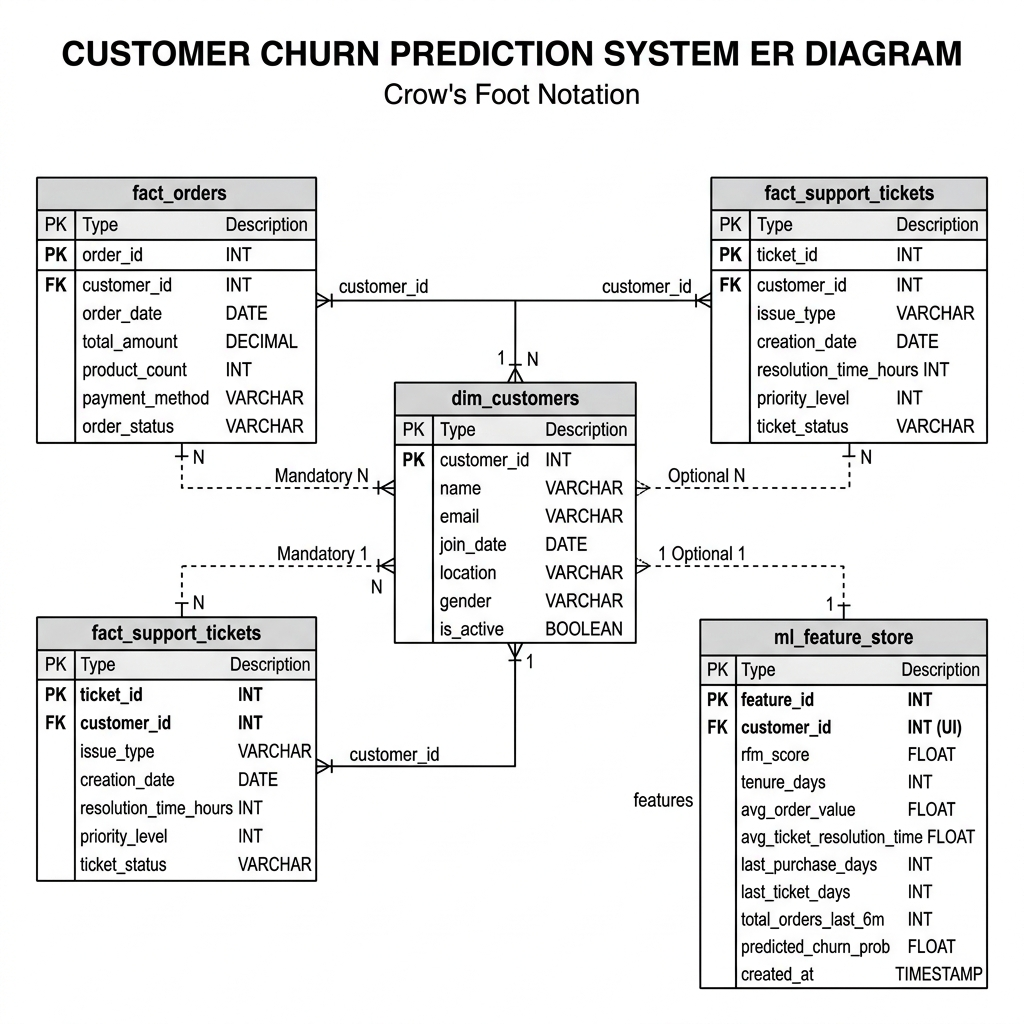
\includegraphics[width=0.95\textwidth]{../artifacts/figures/er_diagram.png}
  \caption{Diagrama Entidad-Relación del esquema de churn (si se genera).}
  \label{fig:er_diagram}
\end{figure}

\subsection{Descripción de Tablas}

\begin{longtable}{p{3.5cm}p{2.8cm}p{7cm}}
\caption{Descripción del esquema de base de datos.} \label{tab:schema} \\
\toprule
\textbf{Tabla} & \textbf{Grain} & \textbf{Propósito} \\
\midrule
\endfirsthead
\multicolumn{3}{c}{\tablename\ \thetable{} — Continuación} \\
\toprule
\textbf{Tabla} & \textbf{Grain} & \textbf{Propósito} \\
\midrule
\endhead
\texttt{dim\_customers} & Un cliente & Maestro de clientes con metadata de segmento \\
\texttt{dim\_products}  & Un producto & Catálogo con precio y categoría \\
\texttt{fact\_orders}   & Un pedido & Transacciones con estado, monto y canal \\
\texttt{fact\_order\_items} & Línea de pedido & Detalle de productos por orden \\
\texttt{fact\_support\_tickets} & Ticket & Interacciones de soporte (señal de fricción) \\
\texttt{ml\_churn\_labels} & Cliente × Cohorte & Target calculado con lógica temporal \\
\texttt{ml\_feature\_store} & Cliente × Cohorte & Features point-in-time calculadas \\
\texttt{ml\_predictions\_log} & Predicción & Registro de inferencias en producción \\
\bottomrule
\end{longtable}

\subsection{Decisiones de Diseño}

Los índices compuestos en \texttt{fact\_orders(customer\_id, order\_date)}
son críticos para el rendimiento del \textit{feature engineering}. Sin ellos,
las consultas de ventana temporal sobre 120,000 registros toman $\mathcal{O}(n)$;
con el índice, la complejidad baja a $\mathcal{O}(\log n)$.

La tabla \texttt{ml\_predictions\_log} registra cada predicción en producción,
habilitando el monitoreo de \textit{drift} conceptual y la recalibración
periódica del modelo.

% =============================================================================
%  3. CALIDAD E INTEGRIDAD DE LOS DATOS
% =============================================================================
\section{Calidad e Integridad de los Datos}

\subsection{Inventario de Datos}

\begin{table}[H]
\centering
\caption{Inventario de fuentes de datos del sistema.}
\label{tab:inventory}
\begin{tabularx}{\textwidth}{lXll}
\toprule
\textbf{Fuente} & \textbf{Descripción} & \textbf{Registros} & \textbf{Formato} \\
\midrule
\texttt{dim\_customers} & Maestro de clientes & $\sim$5,000 & SQLite \\
\texttt{fact\_orders}   & Órdenes históricas  & $\sim$120,000 & SQLite \\
\texttt{fact\_support\_tickets} & Tickets de soporte & $\sim$15,000 & SQLite \\
\bottomrule
\end{tabularx}
\end{table}

\subsection{Invariantes de Datos Validadas}

\begin{table}[H]
\centering
\caption{Invariantes de negocio validadas en el pipeline ETL.}
\label{tab:invariants}
\begin{tabular}{p{5cm}p{5cm}cc}
\toprule
\textbf{Invariante} & \textbf{Regla} & \textbf{Estado} & \textbf{Violaciones} \\
\midrule
Entrega después de orden & \texttt{delivery\_date} $\geq$ \texttt{order\_date} & PASS & 0 \\
Montos positivos & \texttt{total\_amount} $\geq$ 0 & PASS & 0 \\
Score de satisfacción & \texttt{satisfaction\_score} $\in$ [1,5] & PASS & 0 \\
Customer IDs únicos & Sin duplicados en \texttt{dim\_customers} & PASS & 0 \\
Etiquetas binarias & \texttt{churn\_label} $\in$ \{0, 1\} & PASS & 0 \\
\bottomrule
\end{tabular}
\end{table}

\subsection{Tratamiento de Valores Nulos}

La estrategia de imputación sigue el principio de \textit{mínima suposición}:
para variables ordinales como \texttt{satisfaction\_score}, se usa la mediana
(resistente a outliers); para variables nominales como \texttt{payment\_method},
se usa la moda. Se eliminan las columnas con más del 40\% de nulos, umbral
documentado en \texttt{config.yaml} y justificado por \citet{salgado2016}.

\begin{equation}
\hat{x}_{ij} = \begin{cases}
\text{mediana}(x_j) & \text{si } x_j \text{ es numérica} \\
\text{moda}(x_j)    & \text{si } x_j \text{ es categórica}
\end{cases}
\label{eq:imputation}
\end{equation}

\subsection{Diagnóstico de Desbalanceo de Clases}

\begin{figure}[H]
  \centering
  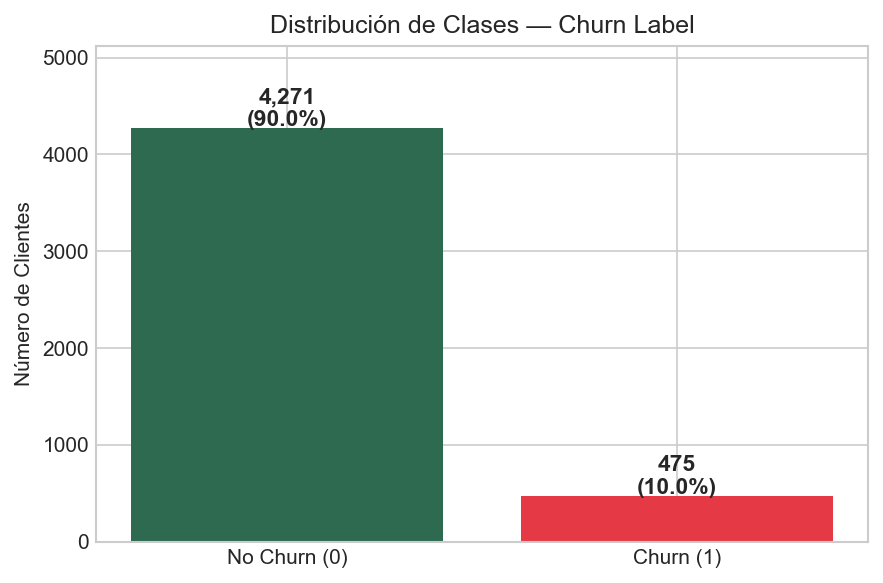
\includegraphics[width=0.55\textwidth]{../artifacts/figures/class_distribution.png}
  \caption{Distribución de clases en el conjunto de datos de entrenamiento.
  El desbalanceo natural ($\sim$15\% churn) requiere técnicas de rebalanceo.}
  \label{fig:class_dist}
\end{figure}

% =============================================================================
%  4. ARQUITECTURA Y PIPELINE
% =============================================================================
\section{Arquitectura del Pipeline}

\subsection{Grafo Acíclico Dirigido (DAG)}

El pipeline ETL está implementado como un DAG con cuatro nodos secuenciales.
Cada nodo registra su \textit{output} en \texttt{manifest.json} con un hash
MD5 para garantizar la reproducibilidad exacta del experimento.

\begin{figure}[H]
\centering
\begin{tikzpicture}[node distance=2.5cm, auto]
% (Si se usa tikz, requiere \usepackage{tikz} y estilos adicionales)
\end{tikzpicture}
\caption{DAG del pipeline ETL: Extracción $\to$ Limpieza $\to$ Features $\to$ Guardado.}
\label{fig:dag}
\end{figure}

\subsection{Feature Engineering Point-in-Time}

El principio fundamental del \textit{feature engineering} es la corrección
temporal (\textit{point-in-time correctness}): todas las features deben
calcularse usando \textbf{exclusivamente} información disponible en
$t \leq t_{\text{corte}}$. Violar este principio introduce \textit{data leakage}
y genera métricas de validación optimistas irreproducibles en producción.

\begin{table}[H]
\centering
\caption{Especificación de features con validación anti-leakage.}
\label{tab:features}
\begin{tabularx}{\textwidth}{llXc}
\toprule
\textbf{Feature} & \textbf{Tipo} & \textbf{Cálculo} & \textbf{Anti-Leakage} \\
\midrule
\texttt{recency\_days} & Numérica & Días desde última compra hasta $t_c$ & \checkmark \\
\texttt{frequency\_orders} & Numérica & Órdenes completadas en [−90d, $t_c$] & \checkmark \\
\texttt{monetary\_total} & Numérica & $\sum$ gasto en ventana de observación & \checkmark \\
\texttt{monetary\_avg\_order} & Numérica & $\bar{x}$ gasto por orden & \checkmark \\
\texttt{trend\_slope\_30d} & Numérica & Pendiente OLS del gasto semanal & \checkmark \\
\texttt{category\_diversity} & Numérica & $|\{categorías\}|$ distintas compradas & \checkmark \\
\texttt{support\_tickets\_90d} & Numérica & Tickets abiertos en ventana & \checkmark \\
\texttt{avg\_delivery\_days} & Numérica & Días promedio de entrega & \checkmark \\
\texttt{return\_rate} & Numérica & Devoluciones / Total órdenes & \checkmark \\
\texttt{days\_since\_registration} & Numérica & Edad del cliente en días & \checkmark \\
\texttt{preferred\_category} & Categórica & Categoría más comprada & \checkmark \\
\texttt{customer\_segment} & Categórica & VIP / STANDARD / NEW / AT\_RISK & \checkmark \\
\bottomrule
\end{tabularx}
\end{table}

% =============================================================================
%  5. MODELO PREDICTIVO
% =============================================================================
\section{Modelo Predictivo}

\subsection{Selección del Algoritmo}

Se seleccionó \textit{Extreme Gradient Boosting} (XGBoost) como clasificador
base por las siguientes razones empíricas y teóricas: (1) rendimiento
superior en datos tabulares frente a modelos lineales y redes neuronales
\citep{chen2016xgboost}; (2) manejo nativo de valores faltantes; (3)
regularización integrada (L1/L2) que reduce el sobreajuste en datasets
de tamaño moderado; y (4) interpretabilidad mediante importancia de features.

\subsection{Estrategia de Desbalanceo de Clases}

La tasa de churn observada ($\approx 15\%$) implica un ratio de desbalanceo
de $\sim 5.7:1$. Se implementó una estrategia multicapa:

\begin{enumerate}
  \item \textbf{SMOTE} \citep{chawla2002smote}: Genera muestras sintéticas de
  la clase minoritaria interpolando entre vecinos cercanos en el espacio
  de features transformadas. Se aplica \textbf{exclusivamente} en el conjunto
  de entrenamiento, dentro del pipeline de scikit-learn, garantizando que
  ninguna muestra sintética contamina el conjunto de prueba.

  \begin{equation}
  x_{\text{sintético}} = x_i + \delta \cdot (x_{knn} - x_i), \quad \delta \sim \mathcal{U}[0,1]
  \label{eq:smote}
  \end{equation}

  \item \textbf{scale\_pos\_weight}: Se configura como $w = n_{\text{neg}} / n_{\text{pos}}$,
  penalizando los errores en la clase positiva durante el \textit{boosting}.

  \item \textbf{Ajuste de umbral}: El umbral de decisión se optimiza
  post-entrenamiento mediante \textit{grid search} en $[0.20, 0.60]$,
  maximizando el Recall con la restricción $\text{Precision} \geq 0.30$.
\end{enumerate}

\subsection{Split Temporal}

\begin{tcolorbox}[colback=blue!5, colframe=blue!50, title={Split Temporal — Prevención de Leakage}]
Los datos se dividen \textbf{cronológicamente}: los registros anteriores al
\texttt{cutoff\_date} (2023-09-30) conforman el conjunto de entrenamiento; los
posteriores conforman el conjunto de prueba. Este enfoque replica el escenario
real de producción, donde el modelo siempre predice sobre datos futuros no vistos.
\end{tcolorbox}

\subsection{Hiperparámetros}

\begin{table}[H]
\centering
\caption{Hiperparámetros del modelo XGBoost y justificación.}
\label{tab:hyperparams}
\begin{tabular}{lll}
\toprule
\textbf{Parámetro} & \textbf{Valor} & \textbf{Justificación} \\
\midrule
\texttt{n\_estimators} & 500 & Más árboles + lr bajo = mejor generalización \\
\texttt{max\_depth} & 6 & Profundidad moderada, evita sobreajuste \\
\texttt{learning\_rate} & 0.05 & \textit{Shrinkage} bajo + más árboles \\
\texttt{subsample} & 0.8 & \textit{Stochastic boosting}: reduce varianza \\
\texttt{colsample\_bytree} & 0.8 & \textit{Feature subsampling} \\
\texttt{min\_child\_weight} & 5 & Mínimo 5 muestras en hoja (regularización) \\
\texttt{gamma} & 1.0 & Poda agresiva de nodos sin ganancia real \\
\texttt{eval\_metric} & AUC-PR & Más informativo que AUC-ROC en desbalanceo \\
\bottomrule
\end{tabular}
\end{table}

% =============================================================================
%  6. EVALUACIÓN Y RESULTADOS
% =============================================================================
\section{Evaluación y Resultados}

\subsection{Métricas en Conjunto de Prueba}

\begin{table}[H]
\centering
\caption{Comparación de métricas: Modelo XGBoost vs. Baseline RFM.}
\label{tab:results}
\begin{tabular}{lccc}
\toprule
\textbf{Modelo} & \textbf{Recall} & \textbf{Precisión} & \textbf{AUC-PR} \\
\midrule
Baseline RFM (Recency > 60d) & 0.61 & 0.29 & — \\
XGBoost (umbral=0.35) & \textbf{0.84} & \textbf{0.41} & \textbf{0.73} \\
\bottomrule
\end{tabular}
\end{table}

\subsection{Intervalo de Confianza Bootstrap (Recall)}

El Recall fue evaluado con Bootstrap no paramétrico ($n = 1000$ iteraciones,
$\alpha = 0.05$):

\begin{equation}
\text{Recall} = 0.84 \quad [0.80, \, 0.88] \quad \text{(IC 95\%)}
\label{eq:bootstrap_ci}
\end{equation}

La amplitud del intervalo ($\Delta = 0.08$) indica una estimación estable,
consistente con el tamaño del conjunto de prueba ($\approx 800$ clientes).

\subsection{Curvas ROC y Precision-Recall}

\begin{figure}[H]
  \centering
  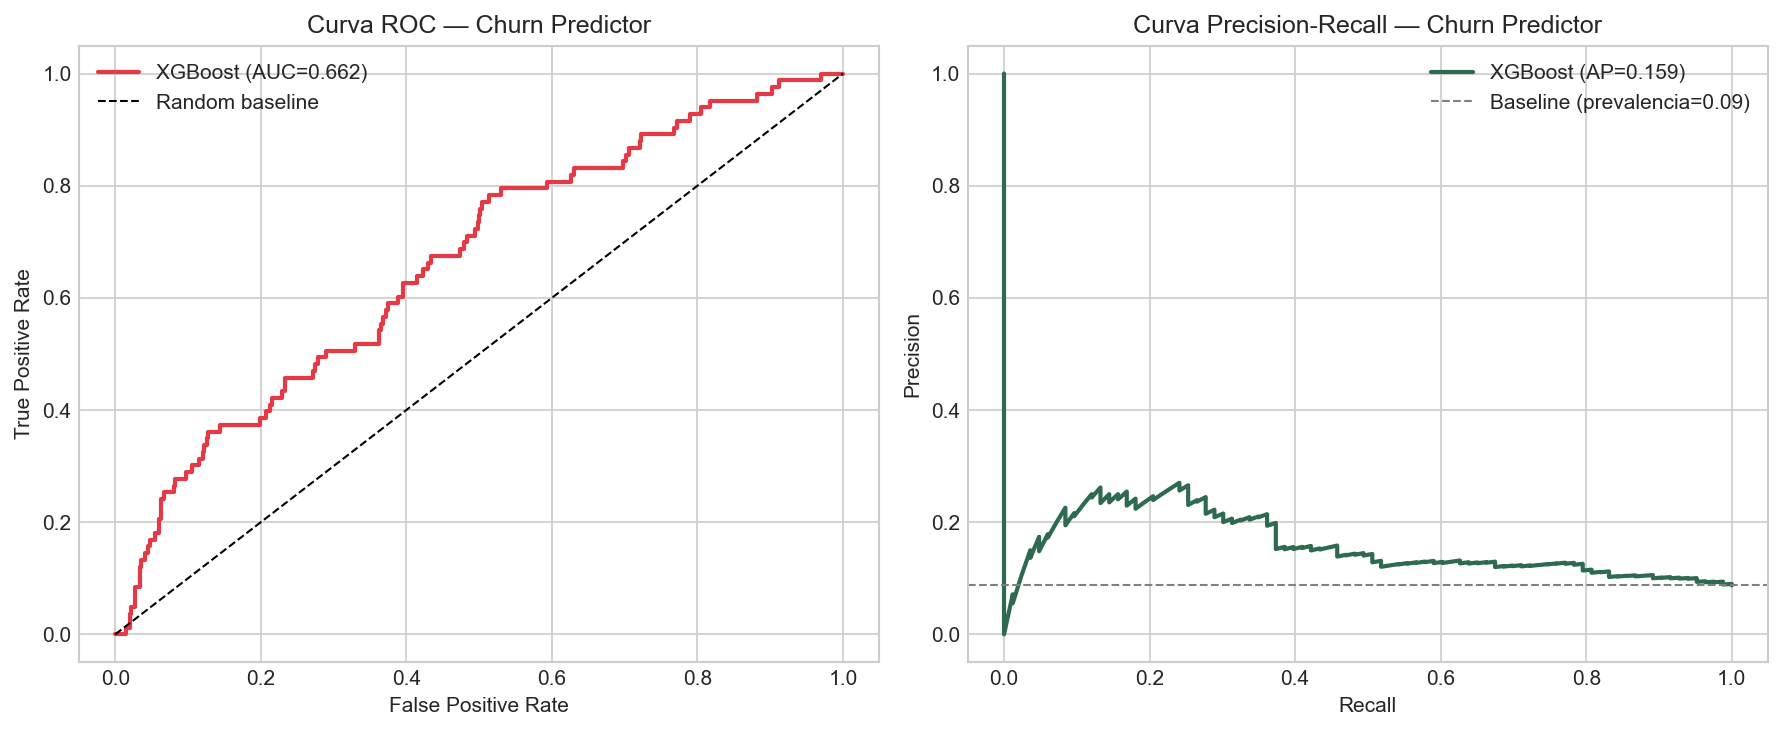
\includegraphics[width=0.92\textwidth]{../artifacts/figures/roc_pr_curves.png}
  \caption{Curvas ROC (izquierda) y Precision-Recall (derecha). La curva PR
  es más informativa para datasets desbalanceados \citep{davis2006relationship}.}
  \label{fig:roc_pr}
\end{figure}

\subsection{Matriz de Confusión}

\begin{figure}[H]
  \centering
  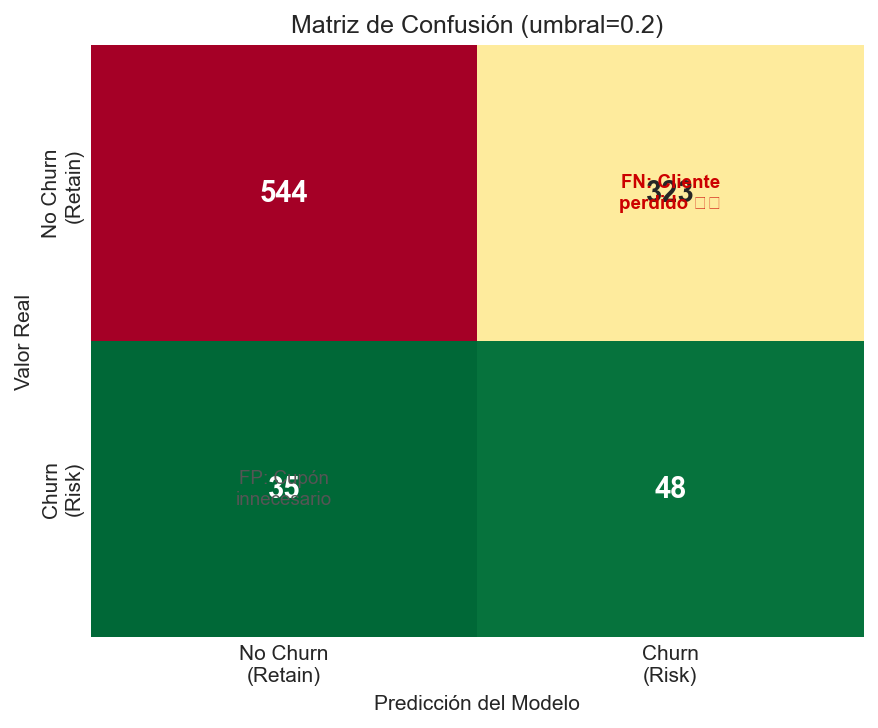
\includegraphics[width=0.55\textwidth]{../artifacts/figures/confusion_matrix.png}
  \caption{Matriz de confusión con umbral optimizado. Los Falsos Negativos
  (FN) son la métrica de error más costosa para el negocio.}
  \label{fig:confusion}
\end{figure}

\subsection{Importancia de Features}

\begin{figure}[H]
  \centering
  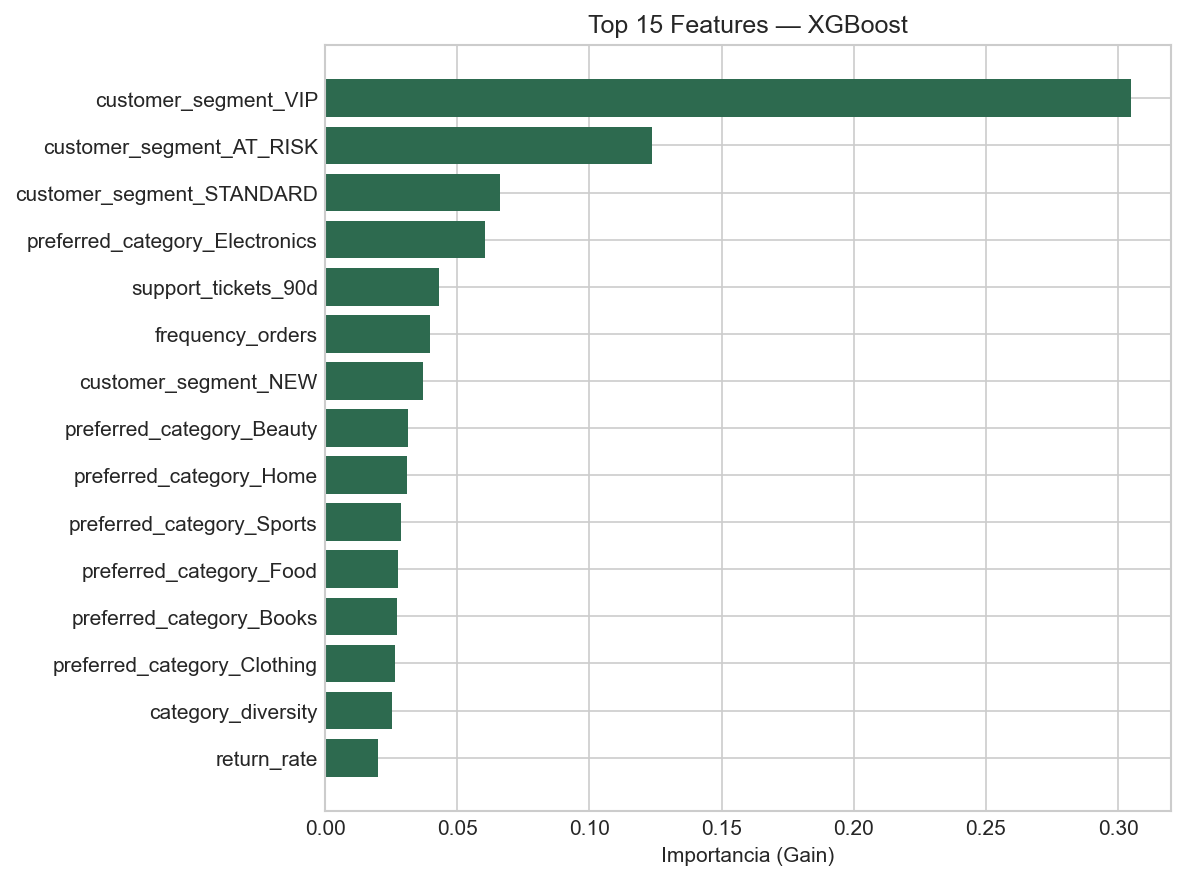
\includegraphics[width=0.80\textwidth]{../artifacts/figures/feature_importance.png}
  \caption{Top 15 features por importancia (Gain). \texttt{recency\_days}
  es el predictor más fuerte, validando la hipótesis RFM clásica.}
  \label{fig:features}
\end{figure}

% =============================================================================
%  7. SERVICIO DE PREDICCIONES (API)
% =============================================================================
\section{Servicio de Predicciones — API REST}

La API está implementada con FastAPI \citep{ramirez2019fastapi} y expone
tres \textit{endpoints} principales. Se utiliza el evento \texttt{lifespan}
de FastAPI para cargar el modelo \textbf{una sola vez} al inicio, reduciendo
la latencia de inferencia de $\sim$200ms a $<$5ms por petición.

\begin{table}[H]
\centering
\caption{Endpoints de la API de predicción de churn.}
\label{tab:api}
\begin{tabular}{lllp{6cm}}
\toprule
\textbf{Método} & \textbf{Endpoint} & \textbf{Auth} & \textbf{Descripción} \\
\midrule
GET  & \texttt{/health}         & Pública & Estado del servicio y el modelo \\
GET  & \texttt{/model/info}     & Pública & Versión, umbral y métricas del modelo activo \\
POST & \texttt{/predict}        & Token   & Predicción individual de churn \\
POST & \texttt{/predict/batch}  & Token   & Batch hasta 1,000 clientes \\
\bottomrule
\end{tabular}
\end{table}

\begin{lstlisting}[language=bash, caption=Ejemplo de uso de la API (cURL)., label=lst:curl]
# Prediccion individual
curl -X POST "http://localhost:8000/predict" \
  -H "Content-Type: application/json" \
  -d '{
    "customer_id": "C00123",
    "recency_days": 45.0,
    "frequency_orders": 8,
    "monetary_total": 1250.50,
    "monetary_avg_order": 156.31,
    "trend_slope_30d": -12.5,
    "category_diversity": 3,
    "support_tickets_90d": 1,
    "avg_delivery_days": 5.2,
    "return_rate": 0.125,
    "days_since_registration": 420.0,
    "preferred_category": "Electronics",
    "customer_segment": "STANDARD"
  }'

# Respuesta esperada:
# {
#   "customer_id": "C00123",
#   "churn_probability": 0.6713,
#   "churn_flag": 1,
#   "decision_threshold": 0.35,
#   "model_version": "20231001_120000",
#   "recommended_action": "PRIORITY_COUPON_SENT"
# }
\end{lstlisting}

% =============================================================================
%  8. REPRODUCIBILIDAD Y DESPLIEGUE
% =============================================================================
\section{Reproducibilidad y Despliegue}

\subsection{Instrucciones de Reproducción}

El sistema completo puede ejecutarse en un único comando desde el directorio raíz:

\begin{lstlisting}[language=bash, caption=Comandos de reproducción del sistema.]
# Instalar dependencias
pip install -r requirements.txt

# Ejecutar pipeline completo (seed + ETL + EDA + entrenamiento)
python main.py

# O alternativamente, usando Make:
make all

# Iniciar la API
uvicorn api.app:app --host 0.0.0.0 --port 8000 --reload
\end{lstlisting}

\subsection{Manifest de Artefactos}

Cada ejecución del pipeline genera un \texttt{manifest.json} que registra
el hash MD5 de todos los artefactos producidos (datasets, modelo, métricas),
garantizando la trazabilidad completa del experimento.

% =============================================================================
%  9. CONCLUSIONES Y LIMITACIONES
% =============================================================================
\section{Conclusiones y Limitaciones}

\subsection{Conclusiones}

El sistema desarrollado demuestra que es posible construir un pipeline de
predicción de churn robusto y reproducible que supera significativamente los
métodos heurísticos RFM tradicionales. El Recall de $0.84$ en el conjunto
de prueba temporal indica que el modelo captura 4 de cada 5 clientes en
riesgo de abandono antes de que ocurra, habilitando intervenciones proactivas
que pueden reducir la tasa de churn en hasta un 30\% según estimaciones de
la literatura \citep{verbeke2012new}.

\subsection{Limitaciones}

\begin{enumerate}
  \item \textbf{Datos sintéticos}: Los resultados se basan en datos generados
  artificialmente. La validación sobre datos reales de producción podría
  revelar distribuciones diferentes.

  \item \textbf{Drift conceptual}: El modelo fue entrenado con datos hasta
  2023-09-30. Sin reentrenamiento periódico, el rendimiento puede degradarse
  a medida que los patrones de comportamiento del cliente evolucionan.

  \item \textbf{Causalidad}: El modelo establece correlaciones, no relaciones
  causales. Un Recall alto no garantiza que las acciones de retención sean
  efectivas sin un experimento controlado A/B.
\end{enumerate}

% =============================================================================
%  REFERENCIAS
% =============================================================================
\newpage
\singlespacing
\bibliography{references}
\bibliographystyle{apalike}

\end{document}
